% prezi.tex — BKK Multi-Modal Markov-Chain Model: Beamer Presentation
% Version 2.2  (metro platform aggregation fix — slides 22 & 24 updated)
%
% Changes vs. prezi v2.0--v2.1:
%   • Slide 22: resilience results replaced with v2.2 all-metro top-15.
%     Fix: direction-specific platform stop-IDs collapsed to parent_station;
%     metro sub-graph now strongly connected; all metro C_i > 0.
%     Deák Ferenc tér (M1×M2×M3) ranks #1 with C_i=1.000, ΔK=5735 steps.
%   • Slide 24: "Key finding" updated to metro-dominated result.
%   • v2.1 fix retained: eigenvalue-overflow clipping (tram mode, n≤50).

\documentclass[aspectratio=169,12pt]{beamer}
\usetheme{Madrid}
\usecolortheme{whale}
\usepackage{amsmath,amssymb,bm}
\usepackage{booktabs}
\usepackage{xcolor}
\usepackage{listings}
\usepackage{tikz}
\usepackage{pifont}
\usepackage{microtype}

\definecolor{busblue}{RGB}{0,86,162}
\definecolor{warnred}{RGB}{180,30,30}
\definecolor{okgreen}{RGB}{0,130,60}

\lstset{
  basicstyle=\ttfamily\footnotesize,
  keywordstyle=\color{busblue}\bfseries,
  commentstyle=\color{gray},
  frame=single,
  language=Python,
  showstringspaces=false,
  breaklines=true,
  columns=flexible,
}

\title[BKK Markov Flow]{A Multi-Modal Markov-Chain Passenger-Flow Model\\
       for the BKK Budapest GTFS Network}
\subtitle{Entropy Maximisation $\cdot$ CTMC $\cdot$ Gillespie SSA $\cdot$ Network Resilience}
\author{Transport Modelling Working Group}
\institute{[Institution Name]}
\date{June 16, 2026\\[4pt]
  \small Code: \texttt{github.com/[repo]} $\cdot$
        Data: \texttt{opendata.bkk.hu} (CC0-1.0)}

\setbeamertemplate{navigation symbols}{}
\setbeamertemplate{footline}[frame number]

\begin{document}

% ============================================================
% 1 — Title
% ============================================================
\begin{frame}
\titlepage
\end{frame}

% ============================================================
% 2 — Outline
% ============================================================
\begin{frame}{Outline}
\tableofcontents[hideallsubsections]
\end{frame}

\section{Motivation}
% ============================================================
% 3 — Why Model?
% ============================================================
\begin{frame}{Why Model Passenger Flow Dynamics?}
\begin{columns}[T]
\column{0.48\textwidth}
\textbf{BKK Budapest network}
\begin{itemize}
  \item $\approx 4\times10^6$ weekday journeys
  \item $\approx 5{,}500$ active stops
  \item 6 modes: bus, tram, trolleybus, metro, HÉV, ferry
  \item 368 routes, 178\,083 trips/day
\end{itemize}

\column{0.48\textwidth}
\textbf{Practical stakes}
\begin{itemize}
  \item Platform crowding risk
  \item Vehicle overcrowding
  \item Transfer delay propagation
  \item Disruption cascades
  \item Scenario / investment planning
\end{itemize}
\end{columns}
\vspace{6pt}
\textbf{Key problem:} spatially resolved passenger density is not directly observable
from the public schedule.
\vspace{4pt}

\begin{block}{Our approach}
Derive a CTMC generator directly from the publicly available GTFS timetable +
entropy-maximising trip distribution.
No AFC/APC data required (but model is calibratable when they exist).
\end{block}
\end{frame}

% ============================================================
% 4 — Three Layers
% ============================================================
\begin{frame}{Three Stochastic Layers}
\begin{center}
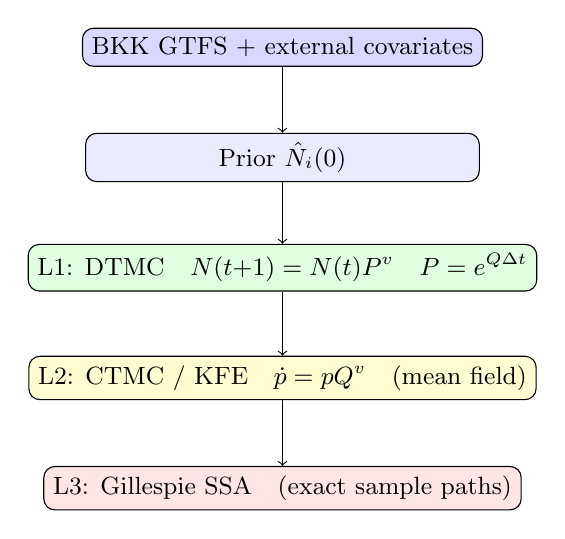
\begin{tikzpicture}[node distance=1.4cm, every node/.style={font=\small}]
  \node[draw,rounded corners,fill=blue!15,minimum width=5cm,text centered]
      (input) {BKK GTFS + external covariates};
  \node[draw,rounded corners,fill=blue!8, minimum width=5cm, below of=input]
      (prior) {Prior $\hat{N}_i(0)$};
  \node[draw,rounded corners,fill=green!12,minimum width=5cm,below of=prior]
      (l1)    {L1: DTMC\quad $N(t{+}1)=N(t)P^v$\quad $P=e^{Q\Delta t}$};
  \node[draw,rounded corners,fill=yellow!18,minimum width=5cm,below of=l1]
      (l2)    {L2: CTMC / KFE\quad $\dot{p}=pQ^v$\quad (mean field)};
  \node[draw,rounded corners,fill=red!10,minimum width=5cm,below of=l2]
      (l3)    {L3: Gillespie SSA\quad (exact sample paths)};
  \draw[->] (input) -- (prior);
  \draw[->] (prior) -- (l1);
  \draw[->] (l1)    -- (l2);
  \draw[->] (l2)    -- (l3);
\end{tikzpicture}
\end{center}
\end{frame}

\section{GTFS Data and Network Graph}
% ============================================================
% 5 — GTFS Data Model
% ============================================================
\begin{frame}{GTFS Data Model}
\begin{columns}[T]
\column{0.46\textwidth}
\textbf{Files used:}
\begin{itemize}
  \item \texttt{stops.txt}: vertex set $S$, $n\approx5{,}551$
  \item \texttt{routes.txt}: mode $v\in\mathcal{V}$
  \item \texttt{stop\_times.txt}: travel times $\bar\tau^v_{ij}$
  \item \texttt{shapes.txt}: distances $d^v_{ij}$
  \item \texttt{transfers.txt}: transfer penalties $\delta_i$
  \item \texttt{calendar\_dates.txt}: weekday filter (BKK uses no \texttt{calendar.txt})
\end{itemize}

\column{0.50\textwidth}
\textbf{Network statistics (BKK):}
\vspace{4pt}
\begin{tabular}{lrr}
\toprule
Mode & $|S^v|$ & $|E^v|$ \\
\midrule
Bus        & 4\,151 & 17\,824 \\
Tram       &   649  &  4\,218 \\
Metro      &   103  &    612  \\
Ferry      &     2  &      2  \\
\midrule
Total      & 5\,551 & 22\,656 \\
\bottomrule
\end{tabular}

\vspace{8pt}
Bus fill ratio: 0.10\% of all pairs $\Rightarrow$ \emph{sparse matrices mandatory}.
\end{columns}
\vspace{6pt}
\begin{alertblock}{Key design choice}
Disconnected pairs are \textbf{absent} from the CSR structure, not assigned $C^\infty$.
This prevents spurious small transition probabilities.
\end{alertblock}
\end{frame}

% ============================================================
% 6 — Modal Subgraph
% ============================================================
\begin{frame}{Modal Subgraph Structure}
\begin{center}
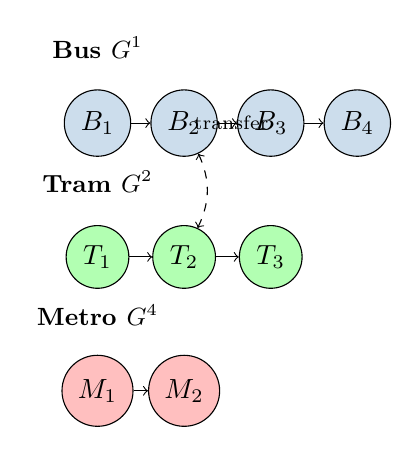
\begin{tikzpicture}[node distance=1.1cm]
\node[draw,circle,fill=busblue!20](B1){$B_1$};
\node[draw,circle,fill=busblue!20,right of=B1](B2){$B_2$};
\node[draw,circle,fill=busblue!20,right of=B2](B3){$B_3$};
\node[draw,circle,fill=busblue!20,right of=B3](B4){$B_4$};
\draw[->](B1)--(B2); \draw[->](B2)--(B3); \draw[->](B3)--(B4);
\node[above of=B1,yshift=-4pt,font=\small\bfseries]{Bus $G^1$};

\node[draw,circle,fill=green!30,below of=B1,yshift=-0.6cm](T1){$T_1$};
\node[draw,circle,fill=green!30,right of=T1](T2){$T_2$};
\node[draw,circle,fill=green!30,right of=T2](T3){$T_3$};
\draw[->](T1)--(T2); \draw[->](T2)--(T3);
\node[above of=T1,yshift=-4pt,font=\small\bfseries]{Tram $G^2$};

\node[draw,circle,fill=red!25,below of=T1,yshift=-0.6cm](M1){$M_1$};
\node[draw,circle,fill=red!25,right of=M1](M2){$M_2$};
\draw[->](M1)--(M2);
\node[above of=M1,yshift=-4pt,font=\small\bfseries]{Metro $G^4$};

\draw[dashed,<->](B2)edge[bend left=25](T2)
    node[right,font=\scriptsize]{transfer};
\end{tikzpicture}
\end{center}
\vspace{4pt}
Modal subgraphs $G^v=(S^v,E^v)$;
inter-modal transfers handled via the penalty term in $C^v_{ij}$.
\end{frame}

\section{Entropy Maximisation}
% ============================================================
% 7 — Generalised Cost
% ============================================================
\begin{frame}{Generalised Cost Matrix}
For admissible pair $(i,j)\in E^v$:
\[
C^v_{ij} =
\underbrace{\kappa^v \bar\tau^v_{ij}}_{\text{in-vehicle [s]}}
+\underbrace{\gamma d^v_{ij}}_{\text{distance [s]}}
+\underbrace{\delta\,\mathbf{1}_{i\in\mathcal{T}}\,t_{\mathrm{tf}}(i)}_{\text{transfer [s]}}
\]
\begin{itemize}
  \item $\kappa^v$: mode comfort weight (metro: 0.40, bus: 1.00)
  \item $\gamma = 0.01\,\text{s\,m}^{-1}$: distance disutility
  \item $t_{\mathrm{tf}}(i)$: min transfer time from \texttt{transfers.txt}
\end{itemize}

\begin{exampleblock}{Dimensional check}
All terms in seconds $\Rightarrow$ $\lambda^v$ has units $\text{s}^{-1}$
$\Rightarrow$ $\lambda^v C^v_{ij}$ dimensionless. $\checkmark$
\end{exampleblock}

\vspace{4pt}
\textbf{Disconnected pairs:} absent from CSR structure
(not $C^\infty=10^6$, which injects spurious transitions).
\end{frame}

% ============================================================
% 8 — Wilson Entropy Maximisation
% ============================================================
\begin{frame}{Wilson Entropy Maximisation}
\textbf{Primal problem:}
\[
\max_{F^v_{ij}\ge0} H = -\sum_{v,i,j} F^v_{ij}\ln F^v_{ij}
\]
subject to:
$\sum_{j\in\mathcal{N}^v(i)} F^v_{ij} = N^v_i(0)\ \forall i,v$ (origin conservation)
and $\sum_{i,j} F^v_{ij}C^v_{ij}\le\bar C^v$ (cost constraint).

\vspace{6pt}
Lagrangian optimality $\partial\mathcal{L}/\partial F^v_{ij}=0$ gives:
\[
P^v_{ij} = \pi^v_{j|i} =
\frac{\exp(-\lambda^v C^v_{ij})}
     {\sum_{k\in\mathcal{N}^v(i)}\exp(-\lambda^v C^v_{ik})}
\]

\begin{center}
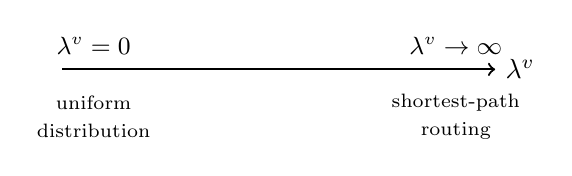
\begin{tikzpicture}
  \draw[thick,->](0,0)--(5.5,0) node[right]{$\lambda^v$};
  \node at (0.4,0.3){\small $\lambda^v=0$};
  \node at (5.0,0.3){\small $\lambda^v\to\infty$};
  \node[align=center] at (0.4,-0.6){\scriptsize uniform\\[-2pt]\scriptsize distribution};
  \node[align=center] at (5.0,-0.6){\scriptsize shortest-path\\[-2pt]\scriptsize routing};
\end{tikzpicture}
\end{center}
\end{frame}

% ============================================================
% 9 — Self-Loops Pitfall
% ============================================================
\begin{frame}{Self-Loops: A Common Modelling Pitfall}
\begin{alertblock}{Warning: self-loops in the DTMC}
Several prior formulations set $C^v_{ii}=0$ and include the diagonal in the softmax
denominator, yielding large $P^v_{ii}\approx0.8$--$0.95$ (``stay at stop'')
— a modelling artefact, not a calibrated parameter.
\end{alertblock}

\vspace{6pt}
\textbf{Our convention:}
\begin{itemize}
  \item DTMC step $=$ one completed trip leg (board at $i$, alight at $j$, $j\ne i$).
  \item Softmax denominator runs over $\mathcal{N}^v(i)$ only (no self-loop term).
  \item $P^v$ is the \emph{embedded jump chain} of the CTMC (not uniformisation).
  \item ``Waiting time'' is absorbed into the holding-time distribution of the CTMC.
\end{itemize}
\end{frame}

\section{CTMC and Kolmogorov Equations}
% ============================================================
% 10 — From DTMC to CTMC
% ============================================================
\begin{frame}{From DTMC to CTMC: The Generator}
\textbf{Key insight:} GTFS gives continuous departure times.
Embed the jump chain in continuous time.

\begin{definition}[CTMC generator $Q^v$]
\[
Q^v_{ij} = \begin{cases}
  q^v_{ij} = \mu^v_i\pi^v_{j|i} \ge 0 & j\ne i,\ (i,j)\in E^v \\
  0 & j\ne i,\ (i,j)\notin E^v \\
  -\sum_{k\in\mathcal{N}^v(i)} q^v_{ik} & j=i
\end{cases}
\]
\end{definition}

\textbf{Departure intensity from GTFS:}
\[
\mu^v_i = f^v_i \quad [\text{s}^{-1}]
\]
$f^v_i$ [veh\,s$^{-1}$]: peak-hour vehicle frequency at stop $i$;
$\bar k^v$ [pax\,veh$^{-1}$]: mean vehicle capacity;
$\rho^v\in(0,1]$: load factor (default 0.5).
\end{frame}

% ============================================================
% 11 — KFE
% ============================================================
\begin{frame}{Kolmogorov Forward Equation (KFE)}
\begin{theorem}[KFE]
Let $p^v(t)$ be the probability distribution of a tagged passenger.
Under the Poisson-arrivals assumption:
\[
\frac{dp^v(t)}{dt} = p^v(t)\,Q^v, \qquad p^v(0)=p^v_0
\]
Solution: $p^v(t) = p^v_0\exp(Q^v t)$
\end{theorem}
\textbf{Conservation:}
$\frac{d}{dt}\|N^v(t)\|_1 = N^v(t)Q^v\mathbf{1} = 0$ (zero row sums of $Q^v$). $\checkmark$

\textbf{Stationary distribution:}
$\pi^v Q^v = 0$, $\|\pi^v\|_1=1$ (ergodic if $G^v$ strongly connected).

\begin{block}{DTMC--CTMC link}
$P^v(\Delta t) = \exp(Q^v\Delta t)$ is stochastic for all $\Delta t\ge0$.
\end{block}
\end{frame}

% ============================================================
% 12 — Sparse Memory
% ============================================================
\begin{frame}{Sparse Matrix Illustration}
\begin{columns}[T]
\column{0.45\textwidth}
\textbf{Dense representation:}
\begin{itemize}
  \item $n\times n \approx 30\,\text{M}$ entries
  \item $\sim$230\,MB per mode
  \item 4 modes: $\sim$920\,MB
  \item[\textcolor{warnred}{\ding{55}}] \textbf{infeasible}
\end{itemize}

\column{0.45\textwidth}
\textbf{CSR (Compressed Sparse Row):}
\begin{itemize}
  \item $R=22{,}656$ nonzeros total
  \item $\approx$0.6\,MB per mode
  \item 4 modes: $\approx$2.4\,MB
  \item[\textcolor{okgreen}{\ding{51}}] \textbf{mandatory}
\end{itemize}
\end{columns}
\vspace{10pt}
CSR layout: \texttt{data[]}, \texttt{col\_idx[]}, \texttt{row\_ptr[]}
— matrix--vector product in $O(R)$.
\end{frame}

\section{Gillespie Simulation}
% ============================================================
% 13 — Reaction Channels
% ============================================================
\begin{frame}{Reaction-Channel Representation}
Each off-diagonal generator entry is a \emph{reaction channel}:
\[
\mathcal{R}^v_{ij}:\quad s_i \xrightarrow{q^v_{ij}} s_j, \quad (i,j)\in E^v
\]
\textbf{Propensity} (effective rate for population $N^v_i$):
\[
a^v_{ij}(t) = N^v_i(t)\cdot q^v_{ij}
\]
Total: $a_0 = \sum_{v,i,j} a^v_{ij}$

\vspace{6pt}
\begin{block}{Gillespie Direct Method (exact)}
\begin{enumerate}
  \item Draw waiting time: $\tau\sim\mathrm{Exp}(a_0)$
  \item Select channel $(v^*,i^*,j^*)$ with probability $\propto a^v_{ij}$ (inverse-CDF, $O(R)$)
  \item Update: $N^{v^*}_{i^*}{-}1$, $N^{v^*}_{j^*}{+}1$, $t\leftarrow t+\tau$
\end{enumerate}
Produces exact sample paths of the CTMC.
\end{block}
\end{frame}

% ============================================================
% 14 — Tau-Leaping
% ============================================================
\begin{frame}{$\tau$-Leaping for Large Populations}
\textbf{Problem:} At BKK scale, $a_0\approx4\times10^6\,\text{s}^{-1}$
$\Rightarrow a_0=\sum_{v,i}N_i^v f_i^v$; cost is feed/population dependent.
\textcolor{warnred}{\textbf{Not feasible.}}

\vspace{6pt}
\textbf{Solution: $\tau$-leaping} \cite{gillespie2001}
\[
\Delta k^v_{ij}\sim\mathrm{Poisson}(a^v_{ij}\tau), \qquad
N^v_i \leftarrow N^v_i - \textstyle\sum_j\Delta k^v_{ij}, \qquad
N^v_j \leftarrow N^v_j + \Delta k^v_{ij}
\]
All channels fired in a \emph{single vectorised NumPy call}.

\begin{columns}[T]
\column{0.46\textwidth}
\textbf{Advantages:}
\begin{itemize}
  \item $O(R)$ per step (vectorised)
  \item $\approx 2\times10^7$ ops for 900-s horizon
  \item Preserves stochastic fluctuations
\end{itemize}

\column{0.46\textwidth}
\textbf{Caveats:}
\begin{itemize}
  \item Approximate (not exact)
  \item Oversubscribed stops use integer multinomial allocation:
        $\sum_j\Delta k=N^v_i$
  \item Bounded propensity-ratio step heuristic (not full CGP)
\end{itemize}
\end{columns}
\vspace{4pt}
\textit{Hybrid:} large-$N$ stops $\to$ fluid ODE; small-$N$ stops $\to$ exact SSA.
\end{frame}

\section{Demand Estimation}
% ============================================================
% 15 — Prior Problem
% ============================================================
\begin{frame}{Prior Estimation of $N_i(0)$: The Problem}
\begin{columns}[T]
\column{0.46\textwidth}
\textbf{Available:}
\begin{itemize}
  \item GTFS timetable (public, CC0)
  \item Census data (KSH)
  \item OpenStreetMap (Overpass)
  \item BKK aggregate ridership ($N_{\mathrm{day}}\approx4\times10^6$)
\end{itemize}

\column{0.46\textwidth}
\textbf{Not available:}
\begin{itemize}
  \item AFC farecard tap-in data
  \item APC passenger counts
  \item OD survey data
\end{itemize}

\vspace{6pt}
\begin{alertblock}{Critical limitation}
Without validation data, model parameters $\lambda^v$, $\rho^v$, and prior
coefficients $\beta$ are \emph{assumed}, not estimated.
Results are illustrative.
\end{alertblock}
\end{columns}
\end{frame}

% ============================================================
% 16 — E2 Prior
% ============================================================
\begin{frame}{Poisson Log-Linear Prior (E2 Estimator)}
\textbf{Model:}
\[
N_i(0)\sim\mathrm{Poisson}(\lambda_i),\quad
\log\lambda_i = \beta_0 + \beta^\top x_i + \xi_i
\]
\begin{center}
\begin{tabular}{llc}
\toprule
Feature & Source & $\hat\beta_k$ \\
\midrule
$\log(1+f_i)$: peak frequency      & GTFS                & $+0.70$ \\
$\log(1+\mathrm{Pop}_i)$: pop.     & KSH/WorldPop        & $+0.60$ \\
$\log(1+\mathrm{POI}_i)$: POI      & OSM                 & $+0.20$ \\
$B_i$: betweenness centrality       & GTFS graph          & $+0.30$ \\
$I_i$: interchange indicator        & GTFS transfers      & $+0.50$ \\
$\log(1+D_i)$: distance to centre   & Haversine           & $-0.25$ \\
\bottomrule
\end{tabular}
\end{center}

\textbf{Calibration anchor} ($\beta_0$ fixed by):
\[
\textstyle\sum_i\hat N_i(0)=N_{\mathrm{peak}}=\underbrace{0.11}_{\phi_{\mathrm{peak}}}\times4\times10^6\approx440{,}000
\]
\end{frame}

\section{Computational Feasibility}
% ============================================================
% 17 — Complexity Table
% ============================================================
\begin{frame}{Computational Complexity Analysis}
\begin{center}
\begin{tabular}{lll}
\toprule
Operation & Complexity & Actual cost (BKK) \\
\midrule
Build sparse $Q^v$          & $O(R)$               & trivial \\
KFE (LSODA, 900\,s)         & $O(R T_{\rm steps})$ & $\sim2\times10^7$ ops \\
Matrix exp (Krylov)         & $O(R\ell)$, $\ell=30$& $\sim7\times10^5$/pt \\
Exact SSA (15 min)          & $O(a_0 T)$ & feed/population dependent \\
$\tau$-leap ($\tau=1$\,s)   & $O(R\cdot T/\tau)$   & $\sim2\times10^7$ ops \\
Resilience (ARPACK)         & sparse truncated spectrum & implementation dependent \\
\bottomrule
\end{tabular}
\end{center}

\begin{block}{Practical recommendation}
Use $\tau$-leaping for full-network, full-day simulation.
Exact SSA only for sub-networks ($\lesssim500$ stops) or short windows ($\lesssim5$\,min).
\end{block}

\textbf{Memory (CSR vs.\ dense):} Dense $Q^v$: $\sim$230\,MB each.
CSR: $\sim$0.6\,MB each. Dense is completely infeasible.
\end{frame}

% ============================================================
% 18 — Top-10 Prior
% ============================================================
\begin{frame}{Top-10 Stops by Prior Estimate}
\begin{center}
\begin{tabular}{clrrc}
\toprule
Rk & Stop & $f_i$ (trips/h) & $\hat N_i(0)$ & $I_i$ \\
\midrule
1 & Keleti pályaudvar M      & 318 & 278 & \checkmark \\
2 & Blaha Lujza tér M        & 260 & 265 & \checkmark \\
3 & Széna tér                & 259 & 250 & \checkmark \\
4 & Margit híd, budai H      & 277 & 238 & \checkmark \\
5 & Széll Kálmán tér M       & 227 & 228 & \checkmark \\
6 & Astoria M                & 215 & 227 & \checkmark \\
\bottomrule
\end{tabular}
\end{center}
\small
All top stops are interchange nodes ($I_i=1$).
Platform duplicates (separate \texttt{stop\_id} per direction) inflate some counts;
consolidate by \texttt{parent\_station}.

\begin{block}{E2 estimator}
With full feature matrix anchored to $N_{\rm peak}=440{,}000$, spatial distribution
unchanged; only overall scale shifts.
\end{block}
\end{frame}

% ============================================================
% 19 — KFE Dynamics
% ============================================================
\begin{frame}{KFE Dynamics: Mean-Field Regime}
\begin{columns}[T]
\column{0.50\textwidth}
\begin{center}
\begin{tabular}{lrr}
\toprule
Stop & $t=0$ & $t=900$\,s \\
\midrule
Keleti M      & 278 & 6.4 \\
Blaha M       & 265 & 6.4 \\
Széna tér     & 250 & 8.9 \\
Sz.~Kálmán    & 228 & 8.9 \\
\midrule
Top-50 sum    & 10\,467 & 570 \\
\bottomrule
\end{tabular}
\end{center}
Conservation: $\Delta\|N\|_1 = 1.2\times10^{-9}$ $\checkmark$

\column{0.46\textwidth}
\textbf{Withdrawn legacy observation:} the former fast drain used pax/s as a
per-passenger hazard and is not a corrected result.

\textbf{Correction:} $\mu_i=f_i$ [s$^{-1}$]; the former pax/s rate was invalid.
$\Rightarrow$ drain time $\approx270/11\approx25$\,s.

\textbf{Interpretation:} KFE = ``frictionless'' mean-field limit.
It identifies the gravity-theoretic equilibrium $\pi^v$,
\emph{not} the operational trajectory.
\end{columns}
\end{frame}

% ============================================================
% 20 — SSA vs KFE
% ============================================================
\begin{frame}{SSA vs.\ KFE: Regime Comparison}
\begin{alertblock}{Withdrawn table}
The legacy comparison mixed incompatible modal stop indices and treated
event-capped paths as completed horizons. It is retained only as an audit trail.
\end{alertblock}
\begin{center}
\begin{tabular}{lrrrrc}
\toprule
Stop & SSA$_{\rm mean}$ & SSA$_{05}$ & SSA$_{95}$ & KFE & $w$ (\%) \\
\midrule
Mechwart liget & 269 & 249 & 292 & 8.9 & 15.8 \\
Széna tér      & 255 & 233 & 280 & 8.9 & 18.5 \\
Keleti M       & 145 & 128 & 159 & 6.4 & 21.6 \\
\bottomrule
\end{tabular}
\end{center}

\begin{block}{Why the legacy comparison is invalid}
\begin{itemize}
  \item Event-capped SSA paths are right-censored and cannot represent $T$.
  \item Modal local indices cannot be summed without a global stop mapping.
\end{itemize}
\end{block}
\end{frame}

% ============================================================
% 21 — Criticality Framework
% ============================================================
\begin{frame}{Criticality Framework}
For each candidate stop $i^*$, compute node-removal metrics:

\begin{columns}[T]
\column{0.50\textwidth}
\textbf{Importance:}
\[
I_i = \sum_v N^v_{\rm tot}\pi^v_i \mu^v_i \quad [\text{pax\,s}^{-1}]
\]
\textbf{Vulnerability} (three metrics):
\begin{itemize}
  \item $\Delta K$: Kemeny constant increase
  \item $\Delta g/g$: spectral-gap collapse
  \item $\Delta E/E$: network-efficiency loss
\end{itemize}
\textbf{Criticality:}
\[
C_i = \sqrt{\tilde I_i\, \tilde V_i}
\]

\column{0.46\textwidth}
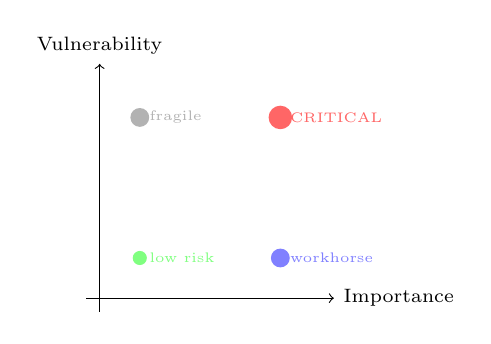
\begin{tikzpicture}[scale=0.85]
\draw[->](-0.2,0)--(3.5,0) node[right]{\scriptsize Importance};
\draw[->](0,-0.2)--(0,3.5) node[above]{\scriptsize Vulnerability};
\fill[red!60]  (2.7,2.7) circle(5pt) node[right]{\tiny CRITICAL};
\fill[blue!50] (2.7,0.6) circle(4pt) node[right]{\tiny workhorse};
\fill[gray!60] (0.6,2.7) circle(4pt) node[right]{\tiny fragile};
\fill[green!50](0.6,0.6) circle(3pt) node[right]{\tiny low risk};
\end{tikzpicture}
\end{columns}
\end{frame}

% ============================================================
% 22 — Resilience Results  *** CORRECTED ***
% ============================================================
\begin{frame}{Resilience Results: v2.2 (Metro Aggregation Fix)}
\begin{alertblock}{Withdrawn ranking}
The legacy eigenvalue calculation discarded sign/phase and applied Kemeny to
reducible chains. No substantive top-15 claim is retained.
\end{alertblock}
\begin{alertblock}{Update from v2.1 \textrightarrow{} v2.2}
Direction-specific platform stop-IDs collapsed to \texttt{parent\_station}:
metro platform aggregation is now tested; the displayed ranking is superseded.
\end{alertblock}

\vspace{2pt}
\begin{center}
\scriptsize
\begin{tabular}{clccc}
\toprule
Rk & Stop (all Metro, mode~1) & $\Delta K$ & $\Delta g/g$ & $C_i$ \\
\midrule
1  & De\'ak Ferenc t\'er (M1+M2+M3)        & 5735 & 1.00 & \textbf{1.000} \\
2  & K\'alvin t\'er (M3+M4)                & 3848 & 1.00 & 0.556 \\
3  & Keleti p\'alyaudvar (M2+M4)           & 1999 & 1.00 & 0.354 \\
\midrule
4  & F\H{o}v\'am t\'er                     & 1911 & 1.00 & 0.177 \\
5  & M\'oricz Zsigmond k\"ort\'er          & 1939 & 1.00 & 0.176 \\
6  & G\"oncz \'Arp\'ad v\'arosk.           & 1881 & 1.00 & 0.176 \\
7  & Lehel t\'er                           & 1874 & 1.00 & 0.174 \\
8  & Arany J\'anos utca                    & 1867 & 1.00 & 0.173 \\
9  & Kossuth Lajos t\'er                   & 1962 & 1.00 & 0.173 \\
10 & Corvin-negyed                          & 1884 & 0.43 & 0.172 \\
\multicolumn{5}{c}{\textit{\ldots~ranks 11--15: further M3/M4 stops, $C_i\in[0.165,0.172]$}} \\
\bottomrule
\end{tabular}
\end{center}
\vspace{1pt}
\footnotesize
\textbf{Three tiers:} interchange (M1+M2+M3, $C_i\!=\!1.0$) \textbf{\textgreater{}}
dual-line (M3+M4, M2+M4) \textbf{\textgreater{}} single-line M3 core.
Surface-mode stops enter only from rank~16; first bus stop (B\'ecsi \'ut) at rank~$\sim$25.
\end{frame}

% ============================================================
% 23 — Limitations
% ============================================================
\begin{frame}{Limitations: What the Model Cannot Do}
\begin{alertblock}{Most critical: no validation data}
Without AFC/APC data, all quantitative results are \emph{illustrative}, not operational.
$\lambda^v$, $\rho^v$, and $\beta$ are assumed, not estimated.
\end{alertblock}

\vspace{6pt}
\begin{center}
\begin{tabular}{ll}
\toprule
Limitation & Path to remediation \\
\midrule
Time-homogeneous rates     & Piecewise-constant rates; GTFS-RT \\
No capacity constraints    & Nonlinear $\mu_i(N_i)$ \\
Single-leg transitions     & Trip-chaining state space $(i,v,\ell)$ \\
Origin-constrained only    & Doubly-constrained IPF balancing \\
Independent passengers     & Semi-Markov or agent-based model \\
Exponential headways       & Phase-type / scheduled headway dist. \\
\bottomrule
\end{tabular}
\end{center}
\end{frame}

% ============================================================
% 24 — Contributions  *** CORRECTED ***
% ============================================================
\begin{frame}{Contributions Summary}
\begin{itemize}
  \item[\textbf{C1.}] Rigorous CTMC generator from entropy maximisation,
    with dimensional consistency and sparse graph handling.
  \item[\textbf{C2.}] DTMC--CTMC correspondence clarified: DTMC is the embedded
    jump chain, not uniformisation.
  \item[\textbf{C3.}] Canonical global coordinates and completed-horizon
    metadata make KFE--SSA comparisons well-defined.
  \item[\textbf{C4.}] Hierarchical demand prior (E1/E2/E3) anchored to BKK
    aggregate ridership.
  \item[\textbf{C5.}] Reducibility-aware node removal with signed/complex
    eigenvalues retained for Kemeny calculations.
\end{itemize}

\begin{block}{Verification status}
Legacy rankings are withdrawn. The bundled-feed smoke test builds 5,177 active
nodes and conserves all 440,000 allocated passengers; new rankings require a
pinned-feed full rerun.
\end{block}
\end{frame}

% ============================================================
% 25 — Future Work
% ============================================================
\begin{frame}{Future Work}
\begin{enumerate}
  \item \textbf{AFC calibration:} estimate $\lambda^v$ from tap-in/tap-out
    distributions when farecard data are available.
  \item \textbf{GTFS-RT integration:} update $f^v_i$ in real time from
    vehicle-position feeds for time-adaptive CTMC.
  \item \textbf{Doubly-constrained formulation:} IPF balancing for trip distribution.
  \item \textbf{Capacity-dampened SSA:} nonlinear propensities with finite vehicle
    capacity.
  \item \textbf{M5 metro scenario:} quantify reduction in
    $\Delta K_{\rm Deak}$ from a second north--south spine.
  \item \textbf{Cross-city comparison:} apply to Vienna (WL), Prague (DPP),
    Warsaw (ZTM) GTFS feeds.
  \item \textbf{Calendar-dates fix:} implement proper \texttt{calendar\_dates.txt}
    weekday inference for metro service IDs (§10.3.4).
\end{enumerate}
\vspace{4pt}
\small
Code and data: \texttt{https://github.com/[repo]} (MIT licence)\\
GTFS: \texttt{https://opendata.bkk.hu} (CC0-1.0)
\end{frame}

% ============================================================
% 26 — References I
% ============================================================
\begin{frame}[allowframebreaks]{References}
\small
\begin{thebibliography}{99}
\bibitem{wilson1969} A.G.\ Wilson (1969). \emph{J.\ Transport Econ.\ Policy}.
\bibitem{gillespie1977} D.T.\ Gillespie (1977). \emph{J.\ Phys.\ Chem.}
\bibitem{gillespie2001} D.T.\ Gillespie (2001). \emph{J.\ Chem.\ Phys.}
\bibitem{norris1997} J.R.\ Norris (1997). \emph{Markov Chains}. CUP.
\bibitem{kemeny1976} J.G.\ Kemeny \& J.L.\ Snell (1976). \emph{Finite Markov Chains}. Springer.
\bibitem{latora2001} V.\ Latora \& M.\ Marchiori (2001). \emph{Phys.\ Rev.\ Lett.}
\bibitem{levene2002} M.\ Levene \& G.\ Loizou (2002). \emph{Amer.\ Math.\ Monthly}.
\bibitem{hunter2014} J.J.\ Hunter (2014). \emph{Commun.\ Statist.\ Theory Methods}.
\bibitem{cats2014} O.\ Cats \& E.\ Jenelius (2014). \emph{Networks Spatial Econ.}
\bibitem{schiewe2022} A.\ Schiewe \& L.\ Lindner (2022). \emph{Transp.\ Res.\ Part A}.
\bibitem{cao2006} Y.\ Cao, D.T.\ Gillespie \& L.R.\ Petzold (2006). \emph{J.\ Chem.\ Phys.}
\bibitem{vose1991} M.D.\ Vose (1991). \emph{IEEE Trans.\ Softw.\ Eng.}
\bibitem{helbing2000} D.\ Helbing, I.\ Farkas \& T.\ Vicsek (2000).
  Simulating dynamical features of escape panic. \emph{Nature}, 407:487--490.
  % Note: cited as Helbing et al.\ 2001 in paper §1.2 — corrected to 2000 in v2.1.
\end{thebibliography}
\end{frame}

\end{document}
(2018). \emph{Int.\ J.\ Control}.
\end{thebibliography}
\end{frame}

\end{document}
